\documentclass[12pt]{report}
\usepackage[utf8]{inputenc}
\usepackage[english]{babel}

\usepackage[letterpaper, margin=15mm]{geometry}
\usepackage{sectsty}
\usepackage[table]{xcolor}
\usepackage[framemethod=tikz]{mdframed} 
\usepackage{wrapfig}
\usepackage{tabularx}
%\usepackage{paralist}
%\usepackage[super,comma,sort&compress,numbers]{natbib}
\usepackage{soul}


\pagenumbering{gobble}

\setlength{\parskip}{1em}

\newmdenv[innerlinewidth=0.5pt,
roundcorner=8pt,
linecolor=gray!20,
innerleftmargin=10pt,
innerrightmargin=10pt,
innertopmargin=10pt,
innerbottommargin=10pt,
backgroundcolor=gray!20
]{highlightbox}

\sectionfont{\large\normalfont\sffamily\bfseries\uppercase}
\subsectionfont{\large\normalfont\sffamily\bfseries}

\newcommand{\project}[1]{\emph{#1}}
\newcommand\Nature{\project{Nature}}
\newcommand\Science{\project{Science}}
\newcommand{\acronym}[1]{#1}
\newcommand\LAMOST{\acronym{LAMOST}}
\newcommand\AAO{\acronym{AAO}}
\newcommand\AAT{\acronym{AAT}}
\newcommand\AAOmega{\acronym{AAOmega}}
\newcommand\APOGEE{\acronym{APOGEE}}
\newcommand\GALAH{\acronym{GALAH}}
\newcommand\BOSS{\acronym{BOSS}}
\newcommand\SEGUE{\acronym{SEGUE}}
\newcommand\SDSS{\acronym{SDSS}}
\newcommand\SDSSV{\SDSS-V}
\newcommand\Kepler{\project{Kepler}}
\newcommand\TESS{\acronym{TESS}}
\newcommand\ESO{\acronym{ESO}}
\newcommand\Gaia{\project{Gaia}}
\newcommand\GES{\Gaia-\ESO}
\newcommand{\todo}[1]{\textcolor{red}{#1}}

\newcommand{\NumStars}{30}
\newcommand{\NumNights}{two grey}

\begin{document}

\section*{The origin of peculiar Mg/K stars throughout the Milky Way}\vspace{-\parskip}

%\textbf{Investigators:} Casey, A.~R. et al.\\
\begin{center}
Casey, A.~R. (PI), Kemp, A.~J., Miles, M.~T., Norfolk, B.~J., Lattanzio, J.~C., Karakas, A.~I.,\\ Schlaufman, K.~C., Ho, A.~Y.~Q., Tout, C.~A., Ness, M., and Ji, A.~P.
\end{center}

% DONT EVER DO THIS SHIT
% BUT I DONT HAVE TIME RN
\newcommand{\refnum}[1]{[#1]}
% Executive summary:

\begin{highlightbox}
Observations reveal that stars in the globular cluster NGC~2419 have potassium abundances three orders of magnitude higher than galactic chemical evolution model predictions, and magnesium abundances an order of magnitude below typical Milky Way values. This abundance signature remains unexplained. Detailed abundances for 5 Mg/K stars in NGC~2419 show that the lighter (e.g., Mg, K, Sc) abundances are correlated with neutron-capture abundances ($Z > 30$), suggesting that either pair-instability supernovae, or super asymptotic giant branch stars with a binary companion, may be responsible. Detailed abundances for more Mg/K stars can be used to test these hypotheses. We have identified 112 stars with  enhanced [K/Fe] and depleted [Mg/Fe] from $\sim$500,000 stars in LAMOST. We request \NumNights\ nights with Subaru/HDS to measure detailed chemical abundances in our brightest \NumStars\ candidates and test hypotheses for the origin of peculiar Mg/K stars.
\end{highlightbox}\vspace{-\parskip}

The production of potassium in the Milky Way is one of the most significant points of tension between observations and galactic chemical evolution models: the predicted level of potassium in the Milky Way is an order of magnitude lower than what is shown by the observations[1]. This discrepancy suggests that there must be other mechanisms, or other nucleosynthetic pathways, that are contributing to the production of potassium in the Milky Way. This deficiency became more notable after observations of NGC~2419 revealed that about half of the stars studied have peculiarly high potassium abundances (up to $[{\rm K/Fe}] = 2$), two orders of magnitude higher than the bulk Milky Way composition at the same metallicity[2,3]. The high abundance ratios of [K/Fe] are complemented by peculiarly low abundance ratios of magnesium ($[{\rm Mg/Fe}] < -1$), an order of magnitude lower than Galactic levels. This extreme signature has, to date, not been observed anywhere else in the Milky Way or its satellites.%\footnote{There are claims that the same abundance signature is observed in NGC~2808[4], but our Figure~\ref{fig:mgk} shows the pattern in NGC~2808 is limited to a mild correlation in Mg-K abundances. Another study[5] reports on a star in the ultra-faint dwarf galaxy Tri~II with the peculiar Mg/K signature, but this claim is disputed by follow-up observations by CI Ji.}

% difficult to make potassium in net quantities, but also difficult to produce  K while depleting  Mg.
%  theoretical attempts failed.

%Observations of NGC~2419 have demonstrated that there is either an exotic and rare event that produces large amounts of potassium, or that there is a significant and unknown nucleosynthetic pathway that is not included in galactic chemical evolution models. In either scenario, it is not known why this mechanism or signature has preferentially occurred in NGC~2419. 





%Detailed chemical abundances of many Mg/K  stars will reveal: (1) if the Mg/K  abundance signature is indeed related  to a peculiar pattern of neutron-capture abundances, and (2) identify the mechanism and conditions that produce this signature.


%We require detailed chemical abundances of many stars showing the Mg/K abundance signature in order to determine (1) if the Mg/K abundance signature is related to a peculiar pattern of neutron-capture abundances, and (2) to understand the mechanisms and conditions that produce this signature. 

\setcounter{figure}{1}
\begin{wrapfigure}{R}{0.35\textwidth}
\begin{center}
	\vspace{-2em}
	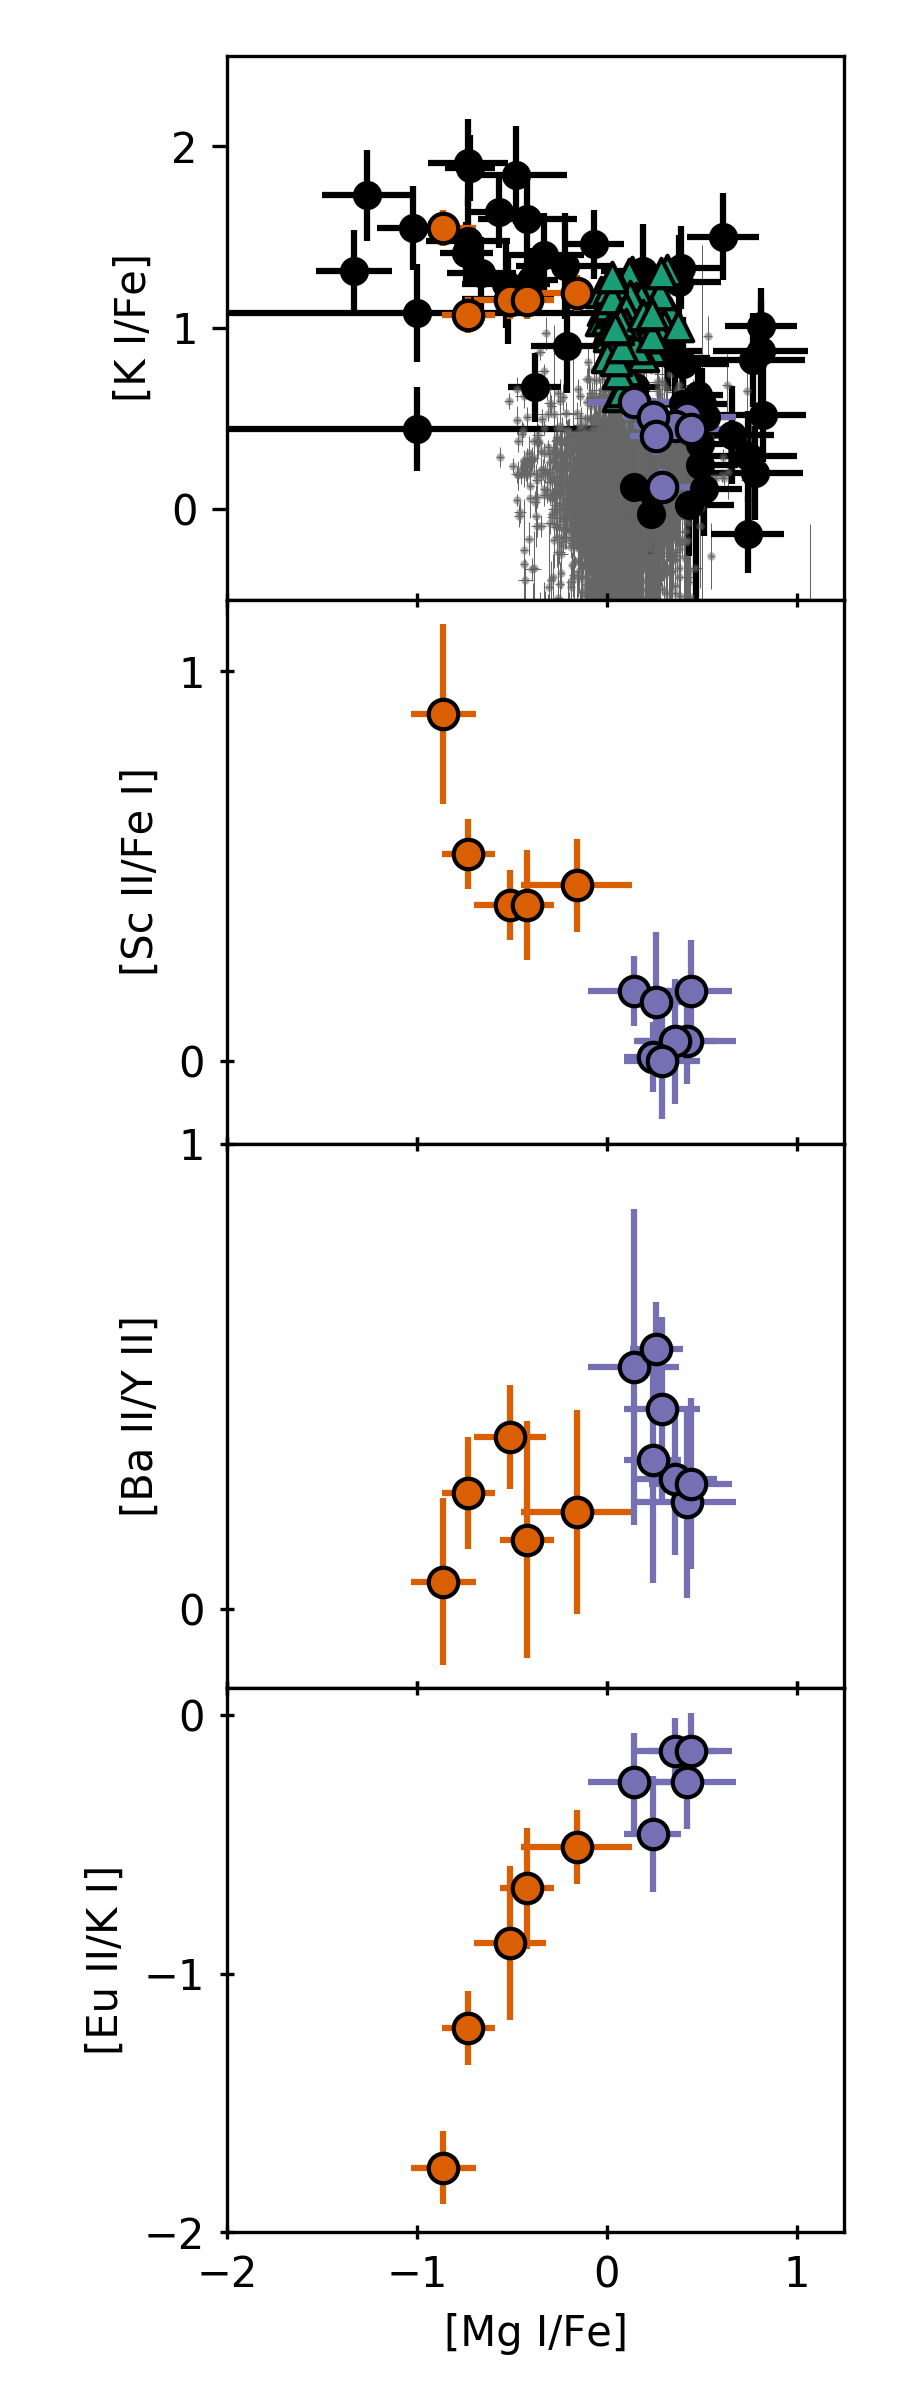
\includegraphics[width=0.35\textwidth]{figures/figure2.png}
	\caption{\small{Detailed chemical abundance ratios (as labelled) for stars in NGC~2419[2,3] and the Milky Way (grey; [7]). Green markers indicate the 112 Mg/K candidates we identified  from LAMOST. Purple and orange markers indicate Mg-normal and Mg-poor populations in NGC~2419[2], respectively, which suggest a relation between light (e.g., Sc, Mg, K) and heavy (e.g., Eu, Ba) elemental abundances.}}
	\vspace{-3em}
	\label{fig:mgk}
\end{center}
\end{wrapfigure}


Theoretical attempts to reproduce the Mg/K signature find that temperatures between 100\,MK and 200\,MK are necessary unless extreme densities are invoked ($>10^8\,{\rm g\,cm}^{-3}$). These calculations, if correct, rule out many mechanisms, including core- and shell-burning of low-mass stars, high-mass and super-massive stars, and normal asymptotic giant branch stars. Two of the potential mechanisms remaining are pair-instability supernovae, and super asymptotic giant branch stars with a binary companion. A large sample of Mg/K stars with detailed chemical abundances are needed to test these hypotheses, including odd-Z (Na, K, Al), $\alpha$-capture elements (Mg, Ca, Ti, Si), Fe-peak (Sc, V, Mn, Ni, Cr, Fe, Cu, Co), and neutron-capture elements (Ba, La, Eu, Y, Ce, Nd).
\setcounter{figure}{0}
\begin{figure}[h!]
	\centering\vspace{-1em}
	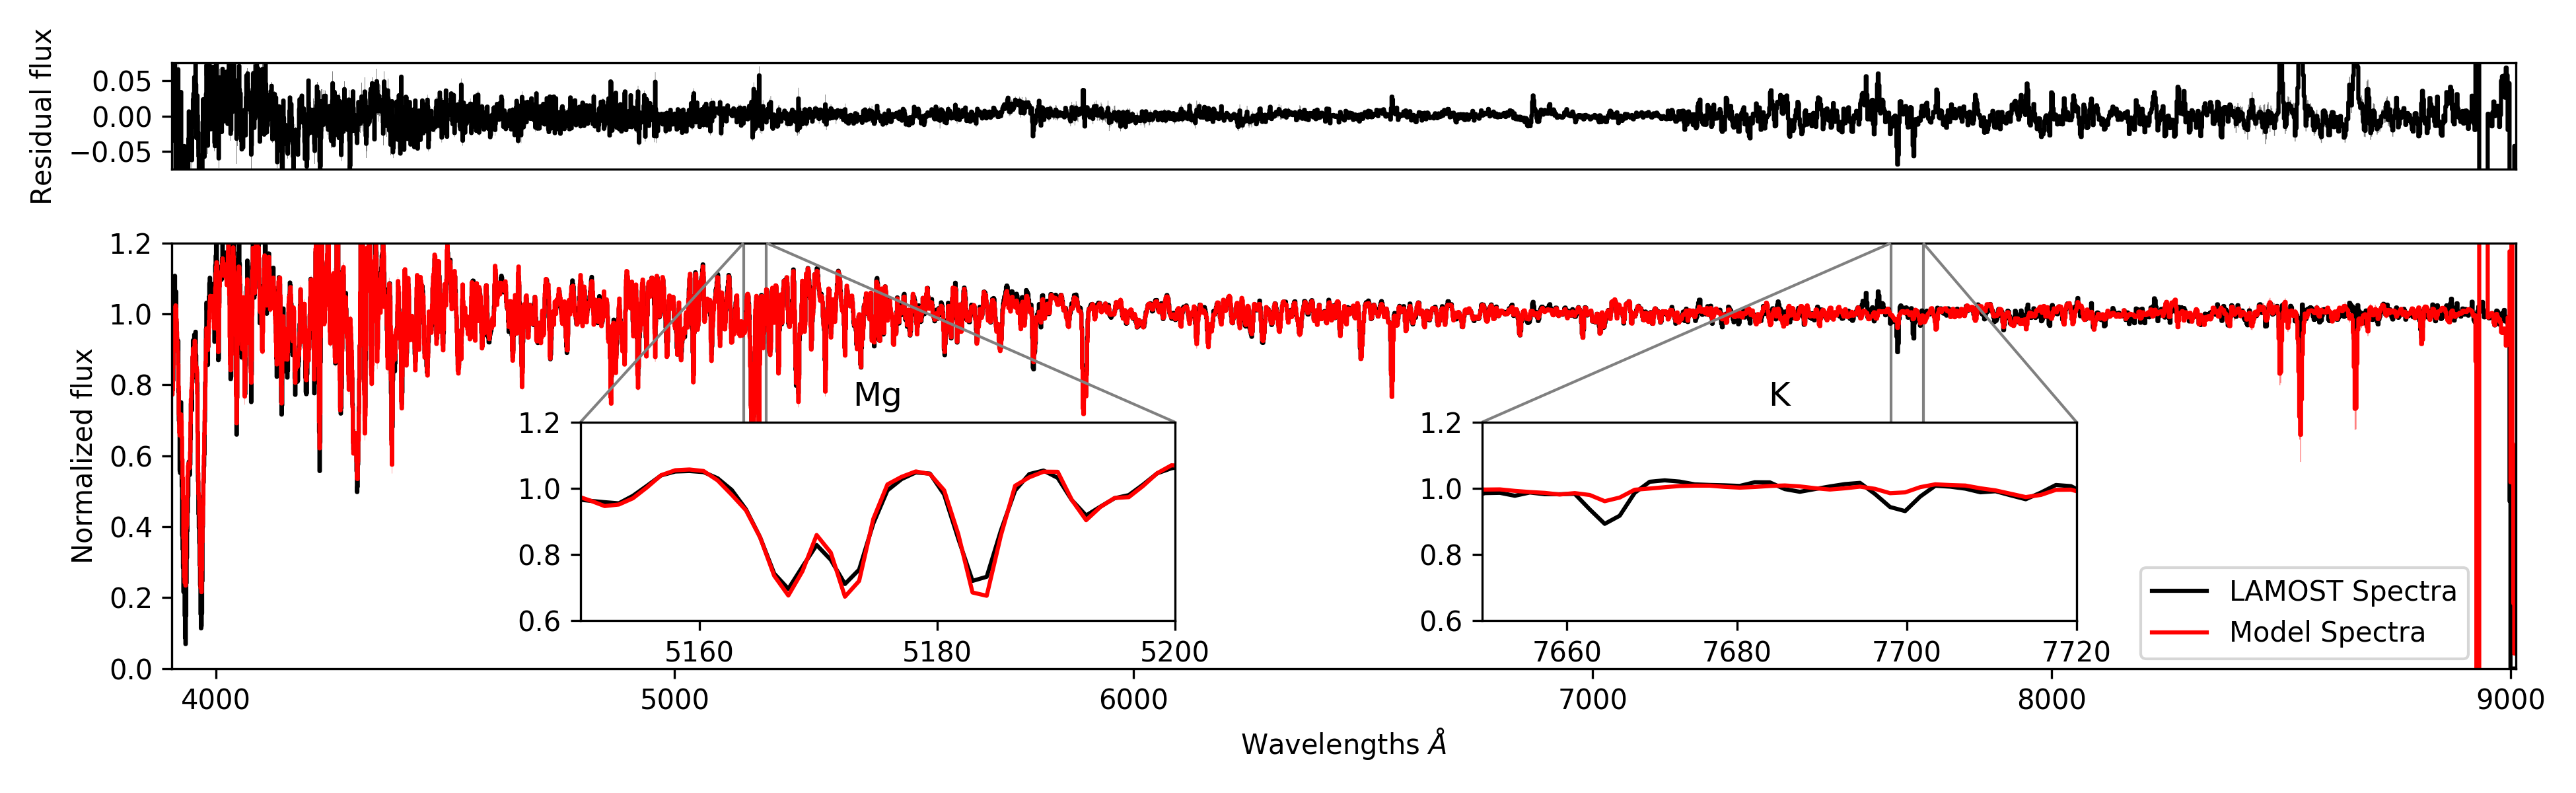
\includegraphics[width=\textwidth]{figures/posterchild.png}
	\vspace{-1em}
\caption{\small LAMOST spectrum (black) and the best-fit data-driven model (red) for a candidate Mg/K star.}\vspace{-2em}
	\label{fig:spectra}\end{figure}


For some  stars in NGC~2419 where high-resolution spectra have been obtained, those data indicate a correlation between the abundances of neutron-capture elements and lighter  elements (Figure 2). Unfortunately the existing sample size is too small to discriminate between hypotheses, and the distance to NGC~2419, 85\,kpc, makes it prohibitively expensive to acquire high signal-to-noise (S/N), high-resolution spectra for a large number of stars.



 We searched the second data release of LAMOST to identify candidate stars that share the Mg/K signature. Specifically we used the data-driven spectrum predictions[6] and a  matched filter algorithm to identify stars with significant flux residuals at the potassium doublet near 766\,nm and the magnesium triplet at 518\,nm. 
 %Our data-driven model includes the stellar parameters $T_{\rm eff}$, $\log{g}$, $[{\rm Fe/H}]$ and $[\alpha/{\rm Fe}]$, and a noise term at each pixel. 
 Conceptually our approach can be described as, for each star, subtracting the median spectrum for stars with similar properties ($T_{\rm eff}$, $\log{g}$, $[{\rm Fe/H}]$ and $[\alpha/{\rm Fe}]$), and identifying flux residuals that are significant above the noise in the data, and above the scatter in flux for stars with similar properties. Any star  with significant flux residuals at the potassium or magnesium lines, above the combined data and model noise, are due to an enhancement or depletion in that element.  We identified 112 highly likely Mg/K candidates from 500,000 giant stars[7] (e.g., see Figure 1).






We propose to observe the brightest \NumStars\ of our candidates during \NumNights\ nights using Subaru/HDS. From these data we will measure detailed chemical abundances of light odd-Z elements (Na, K, Al), $\alpha$-elements (Mg, Ca, Ti, Si), Fe-peak (Sc, V, Mn, Ni, Cr, Fe, Cu, Co), and neutron-capture elements. Those abundance measurements will allow us to confirm if the Mg/K abundance signature is associated with neutron-capture abundance deviations (Figure 2), and to test hypotheses for the origin of this signature. For example, if the Mg/K abundance signature is the result of a pair-instability supernovae, we will recover the characteristic odd-even pattern in the abundances we derive. Alternatively, if we find that the neutron-capture abundances are more consistent with a strong s-process signature, then we will compare the observed abundance signatures to theoretical yields in order to understand the conditions where this signature is produced. Most importantly, a null result here will advance knowledge: confirming that Mg/K stars exist at high [Fe/H] will already be an important scientific result in itself, and if we find that the Mg/K abundance signature is not correlated with a peculiar pattern in other  elements, then it will rule out the two existing hypotheses for the Mg/K abundance signature, and constrain the mechanisms and conditions that are responsible. 

\newcounter{RefCounter}
\setcounter{RefCounter}{1}
\newcommand{\reference}[5]{\small{[\arabic{RefCounter}] #1 \emph{#2} \textbf{#3} #4 (#5).}\stepcounter{RefCounter}}
{\small\noindent
\reference{Kobayashi et al.}{ApJ}{3}{4}{2017}
\reference{Cohen \& Kirby}{ApJ}{760}{86}{2012}
\reference{Mucciarelli et al.}{MNRAS}{426}{2889}{2012}
%\reference{Mucciarelli et al.}{ApJ}{801}{68}{2015}
\reference{Venn et al.}{MNRAS}{466}{3741}{2017}
\reference{Ho et al.}{ApJ}{836}{5}{2017}
\reference{Abolfathi et al.}{ApJS, accepted 28 Nov 2017}{}{arXiv:1707.09322}{2017}
\reference{Kemp et al.}{submitted to MNRAS}{}{}{2018}
}


\end{document}